\chapter{System architecture}
The system architecture is explained in the following chapter.

\section{System description}
The system consists of the following 4 subsystem: The magnetometer, the screen, the GPS module and the ATmega32. Together they form the basic GeoDude system. With the basic system in place, it can show you your current gps location, the time and your heading.\\


\subsection{System block diagram}
The General system can be illustrated by the following block definition diagram:\\
\begin{figure}[H]
	\centering
	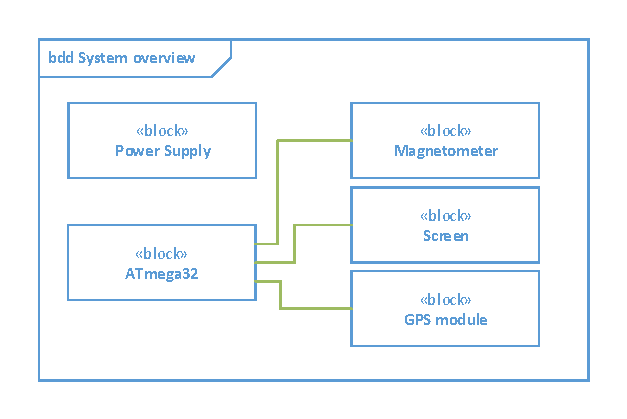
\includegraphics[width=.5\textwidth]{billeder/SystemBDD}
	\caption{Block Definition Diagram of the system}
	\label{bdd:system}
\end{figure}

\section{Behavioural description}
Below is shown a statemachine describing the systems functionality.
\begin{figure}
\centering
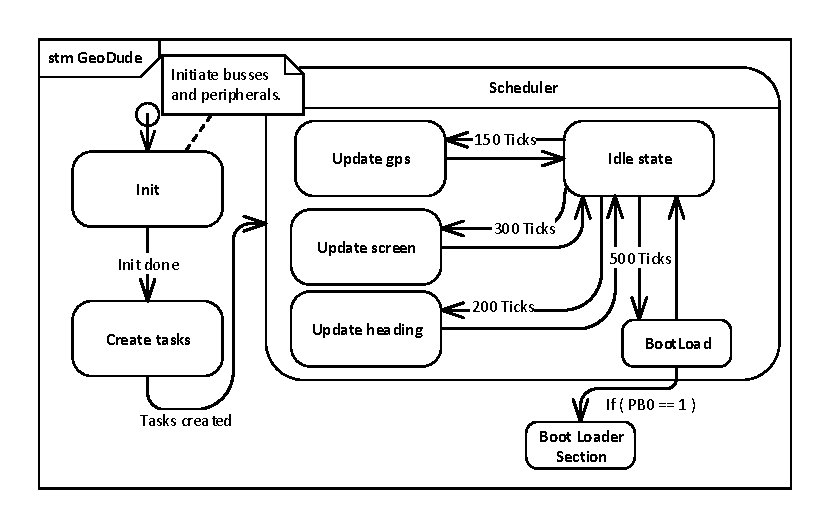
\includegraphics[width=.8\textwidth]{billeder/geodudeSTM}
\caption{GeoDude statemachine}
\end{figure}


\section{Software structure}
The software implemented in this project is described by the UML diagram in the figure below.\\
The system is described via. UML even though it is made in C it offers a nice overview of all headers, variables and function calls.
\begin{figure}[hbpt]
\centering
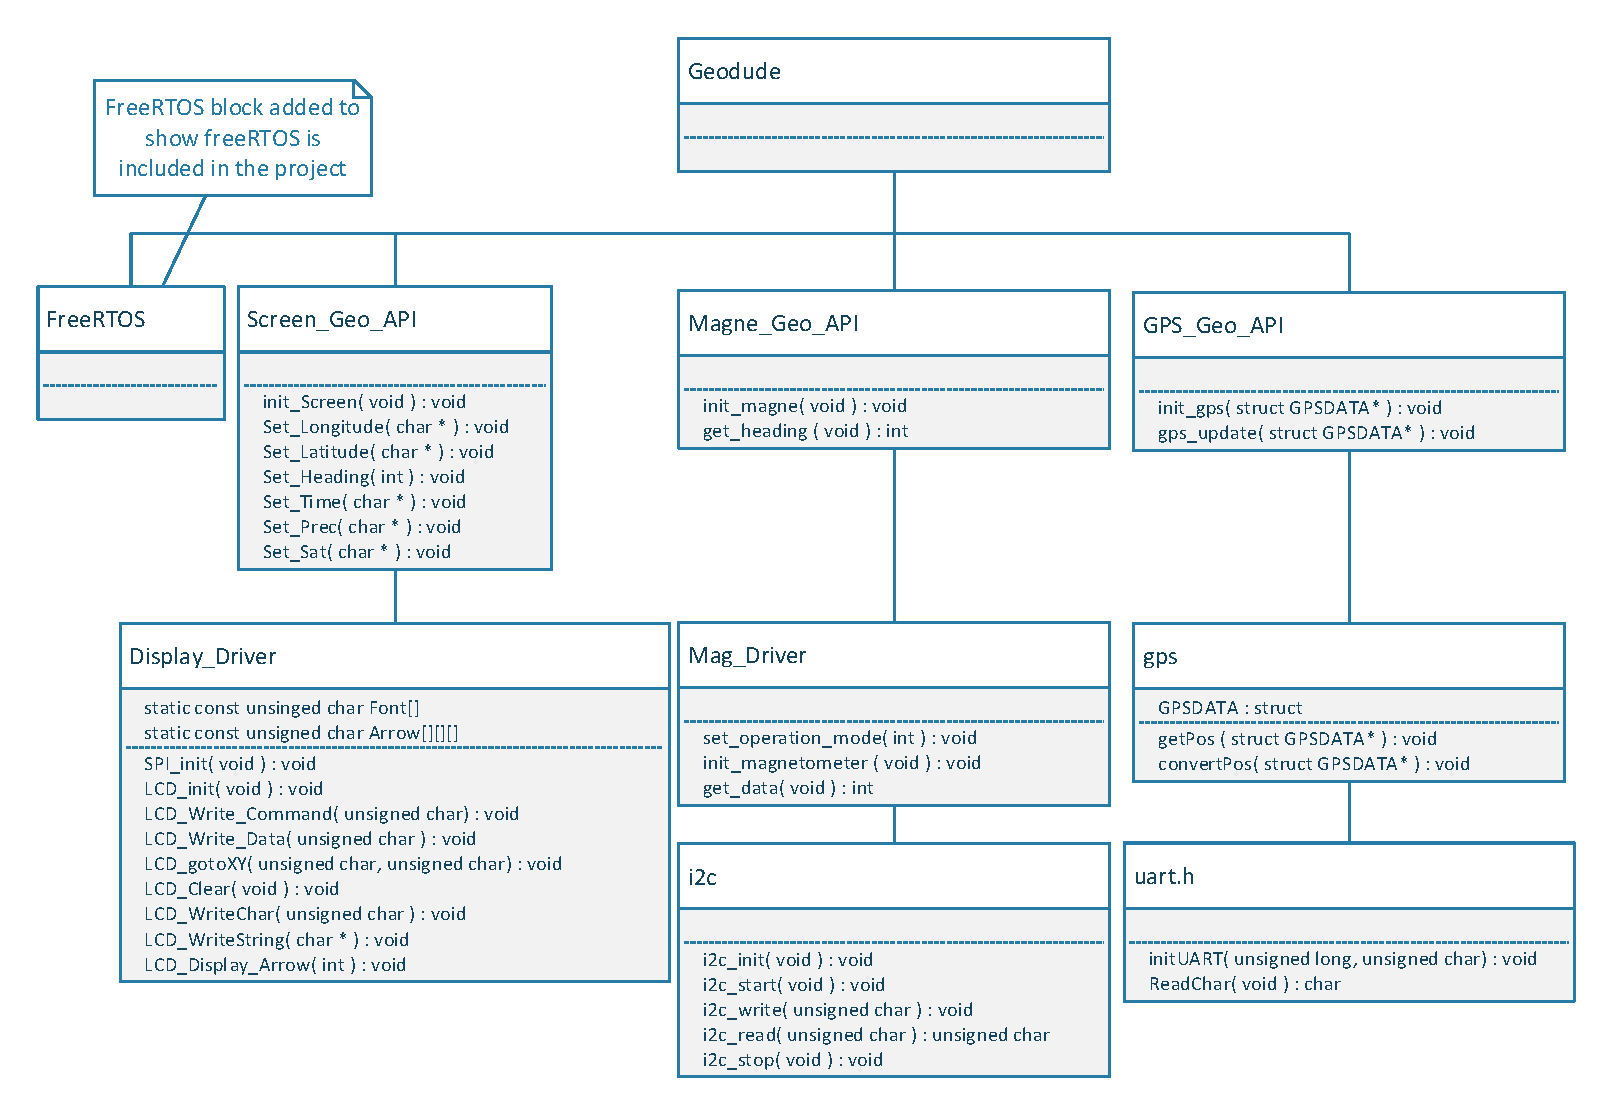
\includegraphics[width=1\textwidth]{billeder/geodude_UML}
\caption{Geodude UML diagram}
\end{figure}


\section{Interfaces/pin assignments}
GeoDude has 3 interfaces, SPI to the screen, I$^2$C to the magnetometer and UART to the GPS receiver.
The following pin assignments have been used:
\begin{table}[H]
\centering
    \begin{tabular}{|l|l|l|l|}
    \hline
    PIN 		& Description    & Levels 	& Unit  \\ \hline
    VCC (10) 	& Supply         & 5 V    	& -		\\ \hline
    GND (11) 	& Ground         & Ground  	& -		\\ \hline
    PA0 (40)	& D/C			 & 0 - 3 V	& Screen \\ \hline
    PA1 (39)	& CS			 & 0 - 3 V  & Screen \\ \hline
    PA2 (38)	& RESET(RST)	 & 0 - 3 V  & Screen \\ \hline
    PB5	(06)	& SPI MOSI		 & 0 - 3 V  & Screen \\ \hline
    PB7 (08)	& SPI CLK		 & 0 - 3 V  & Screen \\ \hline
    PC0 (22) 	& I2C Clock line & 0 - 5 V 	& Magnetometer 	\\ \hline
    PC1 (23) 	& I2C Data line  & 0 - 5 V 	& Magnetometer		\\ \hline
    PD0 (14)	& UART RXD		 & 0 - 5 V	& GPS module \\ \hline
    \end{tabular}
    \caption{Geodude pin assignments}
\end{table}


%\subsection{ATmega32 block diagram}
%The General system can be by the following block definition diagram:\\
%\begin{figure}[H]
%	\centering
%	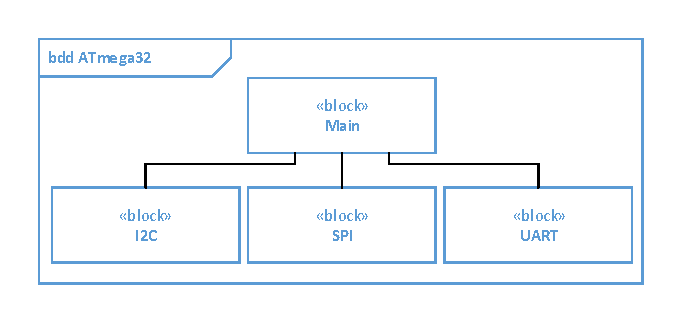
\includegraphics[width=.8\textwidth]{billeder/atmegaBDD}
%	\caption{Block Definition Diagram of the ATmega32}
%	\label{bdd:system}
%\end{figure}
%
%This will lead us to use the following pins:\\
%Logic levels are written as 0 - 5 V.\\
%
%\begin{table}[H]
%\centering
%    \begin{tabular}{|l|l|l|l|}
%    \hline
%    PIN 		& Description    & Levels 	& Unit  \\ \hline
%    VCC (10) 	& Supply         & 5 V    	& -		\\ \hline
%    GND (11) 	& Ground         & Ground  	& -		\\ \hline
%    PA0 (40)	& D/C			 & 0 - 5 V	& Screen \\ \hline
%    PA1 (39)	& CS			 & 0 - 5 V  & Screen \\ \hline
%    PA2 (38)	& RESET(RST)	 & 0 - 5 V  & Screen \\ \hline
%    PB5	(06)	& SPI MOSI		 & 0 - 5 V  & Screen \\ \hline
%    PB7 (08)	& SPI CLK		 & 0 - 5 V  & Screen \\ \hline
%    PC0 (22) 	& I2C Clock line & 0 - 5 V 	& Magnetometer 	\\ \hline
%    PC1 (23) 	& I2C Data line  & 0 - 5 V 	& Magnetometer		\\ \hline
%    PD0 (14)	& UART RXD		 & 0 - 5 V	& GPS module \\ \hline
%    \end{tabular}
%\end{table}
%
%\subsection{Peripherals}
%Logic levels are written as 0 - 5 V or 0 - 3 V.\\
%
%\textbf{The magnetometer:}\\
%\begin{table}[H]
%\centering
%    \begin{tabular}{|l|l|l|}
%    \hline
%    PIN & Description    & Levels  \\ \hline
%    SCL & I2C Clock line & 0 - 5 V \\ \hline
%    SDA & I2C Data line  & 0 - 5 V \\ \hline
%    VCC & Supply         & 5 V     \\ \hline
%    GND & Ground         & Ground  \\ \hline
%    \end{tabular}
%\end{table}
%
%\textbf{The screen:}\\
%\begin{table}[H]
%\centering
%    \begin{tabular}{|l|l|l|}
%    \hline
%    PIN & Description    & Levels  \\ \hline
%    CLK & SPI Clock line & 0 - 3 V \\ \hline
%    DIN & Data in (or MOSI)  & 0 - 3 V \\ \hline
%    VCC & Supply         & 3 V     \\ \hline
%    GND & Ground         & Ground  \\ \hline
%    D/C & Data or Command & 0 - 3 V \\ \hline
%    CS  & Chip Select    & 0 - 3 V \\ \hline
%    RST & Reset			 & 0 - 3 V \\ \hline
%    LED & Background light on display & 3 V \\ \hline
%    \end{tabular}
%\end{table}
%The screen runs on 3 V VCC so all communication from the ATmega32 will have to be voltage divided. 
%
%\textbf{The gps:}\\
%\begin{table}[H]
%\centering
%    \begin{tabular}{|l|l|l|}
%    \hline
%    PIN & Description    & Levels  \\ \hline
%    TX & UART transfer data  & 0 - 5 V \\ \hline
%    VCC & Supply         & 5 V     \\ \hline
%    GND & Ground         & Ground  \\ \hline
%    \end{tabular}
%\end{table}